\documentclass{article}
\usepackage[top=1in, bottom=1in, left=1in, right=1in]{geometry}
% \usepackage{fullpage, fancyhdr}
\usepackage{fullpage}
\usepackage{float}
\usepackage{mathtools}
\usepackage{caption}
\usepackage{subcaption}
\usepackage{portland}
\usepackage{graphicx}
%\usepackage{setspace}
\setlength{\topmargin}{0.0in}
\setlength{\headheight}{0.5in}
\setlength{\headsep}{0in}
\setlength{\footskip}{9pt}

% Use so that included code is pretty
\usepackage{listings}
\usepackage{color}

\definecolor{dkgreen}{rgb}{0,0.6,0}
\definecolor{gray}{rgb}{0.5,0.5,0.5}
\definecolor{mauve}{rgb}{0.58,0,0.82}

\lstset{ %
  backgroundcolor=\color{white},  % choose the background color; you must add \usepackage{color} or \usepackage{xcolor}
  basicstyle=\footnotesize,       % the size of the fonts that are used for the code
  breakatwhitespace=false,        % sets if automatic breaks should only happen at whitespace
  breaklines=true,                % sets automatic line breaking
  captionpos=t,                   % sets the caption-position to bottom
  commentstyle=\color{dkgreen},   % comment style
%   deletekeywords={...},           % if you want to delete keywords from the given language
%   escapeinside={\%*}{*)},         % if you want to add LaTeX within your code
%   extendedchar=false,             % lets you use non-ASCII characters; for 8-bits encodings only, does not work with UTF-8
  frame=single,                   % adds a frame around the code
  keywordstyle=\color{blue},      % keyword style
  language={[x86masm]Assembler},                % the language of the code
  morekeywords={LDR,AREA,ENTRY,CODE,DATA,DCD,SPACE},           % if you want to add more keywords to the set
  numbers=left,                   % where to put the line-numbers; possible values are (none, left, right)
  numbersep=5pt,                  % how far the line-numbers are from the code
  numberstyle=\tiny\color{gray},  % the style that is used for the line-numbers
  rulecolor=\color{black},        % if not set, the frame-color may be changed on line-breaks within not-black text (e.g. comments (green here))
  showspaces=false,               % show spaces everywhere adding particular underscores; it overrides 'showstringspaces'
  showstringspaces=false,         % underline spaces within strings only
  showtabs=false,                 % show tabs within strings adding particular underscores
  stepnumber=1,                   % the step between two line-numbers. If it's 1, each line will be numbered
  stringstyle=\color{mauve},      % string literal style
  tabsize=8,                      % sets default tabsize to 2 spaces
  title=\lstname                  % show the filename of files included with \lstinputlisting; also try caption instead of title
}



% \pagestyle{fancyplain}
\pagestyle{myheadings}
\voffset=-0.50in
\topmargin=0.00in 
\headsep=0.25in 
\evensidemargin=0in 
\oddsidemargin=0in 
\textwidth=6.6in 
\textheight=10.0in 

\renewcommand{\topfraction}{0.9}	% max fraction of floats at top
\renewcommand{\bottomfraction}{0.8}	% max fraction of floats at bottom
%   Parameters for TEXT pages (not float pages):
\setcounter{topnumber}{2}
\setcounter{bottomnumber}{2}
\setcounter{totalnumber}{4}     % 2 may work better
\setcounter{dbltopnumber}{2}    % for 2-column pages
\renewcommand{\dbltopfraction}{0.9}	% fit big float above 2-col. text
\renewcommand{\textfraction}{0.07}	% allow minimal text w. figs
%   Parameters for FLOAT pages (not text pages):
\renewcommand{\floatpagefraction}{0.7}	% require fuller float pages
% N.B.: floatpagefraction MUST be less than topfraction !!
\renewcommand{\dblfloatpagefraction}{0.7}	% require fuller float pages
% remember to use [htp] or [htpb] for placement

\title{Assignment \# 3: Problem Set 2, Problem 1}
\date{1/29/2013}
\author{Brian Arnberg}

\markright{Brian Arnberg\hfill ELEC 6260 - Embedded Computing Systems\hfill}     
\setlength{\parindent}{0pt}


\begin{document}\label{start}

% \begin{titlepage}
	\maketitle
	\thispagestyle{empty}
% \end{titlepage}


% \section*{Assignment \# 3: Problem Set 2, Problem 1}
\section*{Assignment}

For the following, write an ARM assembly language program, and in the Keil MDK-ARM
IDE, create a project, enter the program, and then execute and debug it in the Keil
MDK-ARM debugger. You may run the program either in the simulator or in RAM on the
STM32F4-DISCOVERY board. All program variables are to be 32-bit integers. You may choose
your own test data values.\\

Compute:\\ \texttt{zz = aa*(bb+cc) � (dd*35)}\\
 Place aa,bb,cc,dd in the code area, so that you can provide initial values with "DCD"
 assembler directives. Place zz in the data area, so that you can write the result to it. The
 final debug window should show the final value of zz in memory.

\section*{ Debugging }
The ARM assembly language program was written inside a Linux environment, with the expectation that it would be compiled against an "ARM" version of gcc (\texttt{arm-none-eabi-as}). The compiler did not accept the line labels, and would not compile the code. This lead to the code being debugged on a school computer. The school computers do not have the proper drivers installed to communicate with the STM32F4, so the program was debugged inside the Simulator. Because the program was installed inside the simulator, the Target addresses for the ROM and RAM portions were left at their default values (0x8000000 and 0x20000000, respectively). The ``Memory'' section of the debugger is displayed in Figure~\ref{fig:memory}, and the value of zz has been circled. The expected value for zz is -135, and this is the value stored in the memory location for zz. Therefore, the program worked as expected. 

\begin{figure}
	\centering
	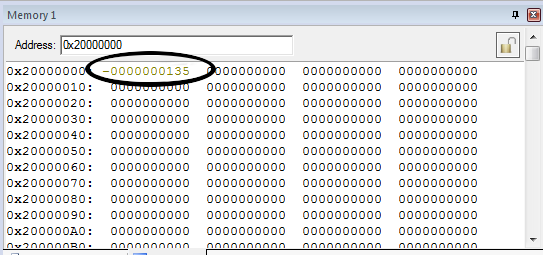
\includegraphics[width=\textwidth,keepaspectratio]{memory}
	\caption{A screen capture of the memory box inside the debugger window. The expected value for zz is $-135$, and this is what is displayed. Therefore, the debugged program indicates that the program works as expected. }
	\label{fig:memory}
\end{figure}

\newpage
\section*{ Source Program }
\lstinputlisting{PS2-1.s}
PS2-1.s is the ARM assembly language program written to compute \texttt{zz = aa*(bb+cc) - (dd*35)}. The values I selected for aa, bb, cc, and dd were 1, 2, 3, and 4, respectively. The expected value for zz is $-135$.



%  \begin{figure}[htbp]
%   \centering
%   \includegraphics[width=4.0in,keepaspectratio]{E-Field}
%   \caption{\small{ The E-Field pattern produced by the initial code. }}
%   \label{fig:E-Field}
%   \end{figure}
%  \begin{figure}[htbp]
%   \centering
%   \includegraphics[width=4.0in,keepaspectratio]{Power}
%   \caption{\small{ The normalized power pattern of the system.  }}
%   \label{fig:Power}
%   \end{figure}

\label{end}\end{document}


